%%%
% Plantilla de Memoria
% Modificación de una plantilla de Latex de Nicolas Diaz para adaptarla 
% al castellano y a las necesidades de escribir informática y matemáticas.
%
% Editada por: Mario Román
%
% License:
% CC BY-NC-SA 3.0 (http://creativecommons.org/licenses/by-nc-sa/3.0/)
%%%

%%%%%%%%%%%%%%%%%%%%%%%%%%%%%%%%%%%%%%%%%
% Thin Sectioned Essay
% LaTeX Template
% Version 1.0 (3/8/13)
%
% This template has been downloaded from:
% http://www.LaTeXTemplates.com
%
% Original Author:
% Nicolas Diaz (nsdiaz@uc.cl) with extensive modifications by:
% Vel (vel@latextemplates.com)
%
% License:
% CC BY-NC-SA 3.0 (http://creativecommons.org/licenses/by-nc-sa/3.0/)
%
%%%%%%%%%%%%%%%%%%%%%%%%%%%%%%%%%%%%%%%%%

%----------------------------------------------------------------------------------------
%	PAQUETES Y CONFIGURACIÓN DEL DOCUMENTO
%----------------------------------------------------------------------------------------
%%% Configuración del papel.
% microtype: Tipografía.
% mathpazo: Usa la fuente Palatino.
\documentclass[a4paper, 11pt]{article}
\usepackage[protrusion=true,expansion=true]{microtype}
\usepackage{mathpazo}

\usepackage{fancyvrb}

% redefine \VerbatimInput
\RecustomVerbatimCommand{\VerbatimInput}{VerbatimInput}%
{fontsize=\footnotesize,
	%
	frame=lines,  % top and bottom rule only
	framesep=2em, % separation between frame and text
	rulecolor=\color{Gray},
	%
	label=\fbox{\color{Black}data.txt},
	labelposition=topline,
	%
	commandchars=\|\(\), % escape character and argument delimiters for
	% commands within the verbatim
	commentchar=*        % comment character
}



% Indentación de párrafos para Palatino
\setlength{\parindent}{0pt}
  \parskip=8pt
\linespread{1.05} % Change line spacing here, Palatino benefits from a slight increase by default




%%% Castellano.
% noquoting: Permite uso de comillas no españolas.
% lcroman: Permite la enumeración con numerales romanos en minúscula.
% fontenc: Usa la fuente completa para que pueda copiarse correctamente del pdf.
\usepackage[spanish,es-noquoting,es-lcroman]{babel}
\usepackage[utf8]{inputenc}
\usepackage[T1]{fontenc}
\selectlanguage{spanish}




%%% Gráficos
\usepackage{graphicx} % Required for including pictures
\usepackage{wrapfig} % Allows in-line images
\usepackage[usenames,dvipsnames]{color} % Coloring code

%%% Matemáticas
\usepackage{amsmath}


%%% Bibliografía
\makeatletter
\renewcommand\@biblabel[1]{\textbf{#1.}} % Change the square brackets for each bibliography item from '[1]' to '1.'
\renewcommand{\@listI}{\itemsep=0pt} % Reduce the space between items in the itemize and enumerate environments and the bibliography

%% ENLACES 
\usepackage{hyperref}
\hypersetup{
	colorlinks   = true,    % Colours links instead of ugly boxes
	urlcolor     = MidnightBlue,    % Colour for external hyperlinks
	linkcolor    = MidnightBlue, %BurntOrange,    % Colour of internal links
	citecolor    = MidnightBlue      % Colour of citations
}

%% codigo


\usepackage{listings}   
\usepackage{xcolor}


%% cosas 

\usepackage[margin=1in]{geometry}

\usepackage{times}


%% colorear titulos
\usepackage{titlesec}
\titleformat{\section}
{\color{MidnightBlue}\normalfont\Large\bfseries}
{\color{Black}\thesection}{1em}{}


%% CREAR DIAGRAMAS 

\usepackage{tikz}

%% rodear figura de texto
\usepackage{graphicx,wrapfig,lipsum}
 %% comentarios multilinea
\usepackage{verbatim}

\definecolor{darkGray}{gray}{0.05}

%----------------------------------------------------------------------------------------
%	DOCUMENTO
%----------------------------------------------------------------------------------------

\begin{document}
	
	
	\begin{titlepage}
		\begin{center}
			\vspace*{0.2cm}
			
			{\Huge \textbf{\textcolor{Black}{ALGORÍTMICA}}}
			
						{\textcolor{MidnightBlue}	{\Huge\underline{PRÁCTICA 1: EFICIENCIA}}}
			
				\vspace{0.2cm}
				
				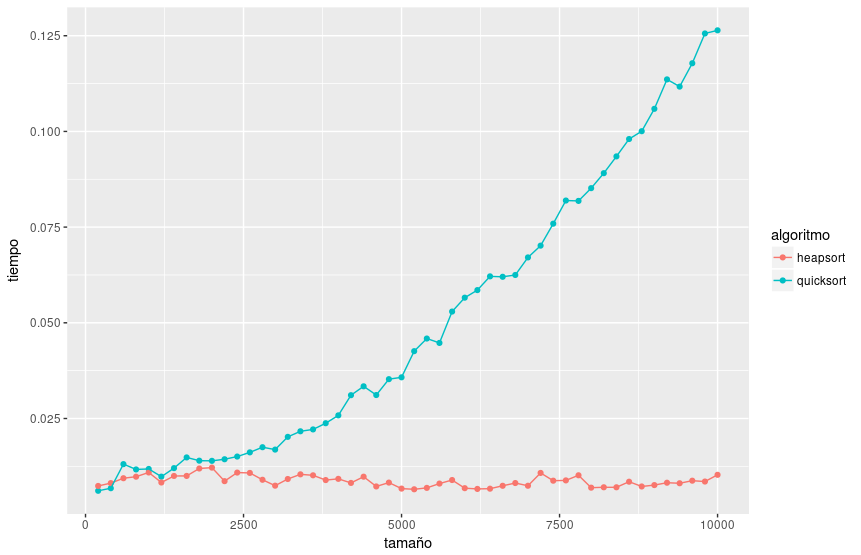
\includegraphics[width=\textwidth]{cover.png}
				\vspace{0.2cm}
				

		
			\vspace{1cm}
			
			\textbf{AUTORES: \\
					Pablo Moreno Megías, Diego Lerena García, Manuel Vallejo Felipe, Ángel Díaz de la Torre, Francisco Navarro Morales, Marcel Kemp Muñoz y David Redondo Correa
		    		 }
	    		 \vspace{1cm}
	   
			
			\vfill
			Algorítmica [PRACTICAS]\\
			Segundo curso del Grado de Ingeniería Informática.\\
			Universidad de Granada.\\
			curso 2016-2017.
		\end{center}
	\end{titlepage}


%\maketitle % Print the title section

%% Resumen (Descomentar para usarlo)
\renewcommand{\abstractname}{Resumen} % Uncomment to change the name of the abstract to something else
%\begin{abstract}
% Resumen aquí
%\end{abstract}

%% Palabras clave
%\hspace*{3,6mm}\textit{Keywords:} lorem , ipsum , dolor , sit amet , lectus % Keywords
%\vspace{30pt} % Some vertical space between the abstract and first section

\color{darkGray}
%% Índice
{\parskip=2pt
  \tableofcontents
}
\pagebreak
\section{Eficiencia empírica}
\subsection{Algoritmos de orden $nlogn$.}
En primer lugar realizamos el análisis empírico de los algoritmos de ordenación de orden $nlogn$. Obtuvimos, con un script, para cada algoritmo los tiempos de ejecución para distintos tamaños y reflejamos los datos obtenidos en gráficas.

\begin{figure}[!hbp]
	 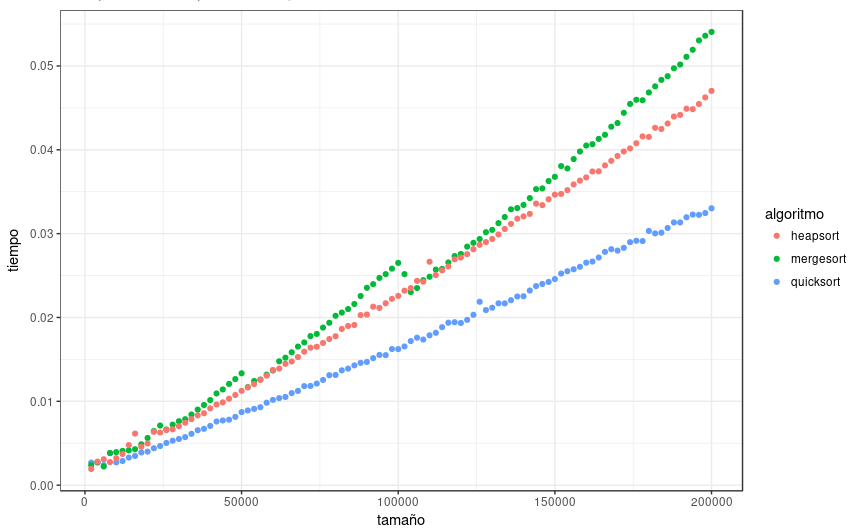
\includegraphics[width=\textwidth]{ordempirica.png}
	\caption{Eficiencia empírica de los algoritmos de ordenación de orden $nlogn$.\label{empiricaor}}
\end{figure}


    Podemos ver como aunque los 3 algoritmos tengan el mismo análisis O, el algoritmo de inserción es más eficiente que los demás y el burbuja el que menos, aunque esto a una gran cantidad de datos se hace insignificante.
\pagebreak
\subsection{Algoritmos de orden $n^2$.}

Del mismo modo, obtuvimos los tiempos empíricos para los algoritmos de ordenación de orden $n^2$ y obtuvimos mejores resultados para el algoritmo de selección.

\begin{figure}[!hbp]
	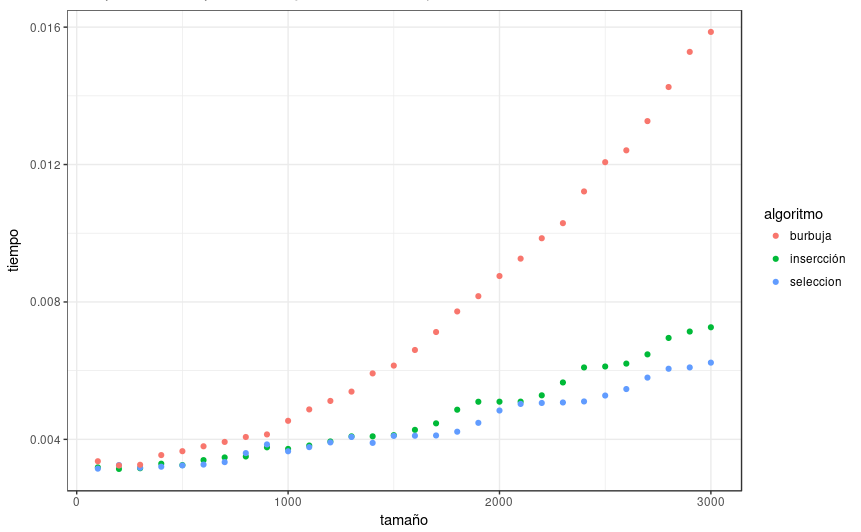
\includegraphics[width=\textwidth]{n2ord.png}
	\caption{Eficiencia empírica de los algoritmos de ordenación de orden $n^2$.\label{n2or}}
\end{figure}

\pagebreak
\subsection{Algoritmo de orden $n^3$.}
El único algoritmo de este orden era el de Floyd. Los tiempos obtenidos se reflejan en la siguiente gráfica:


\begin{figure}[!hbp]
	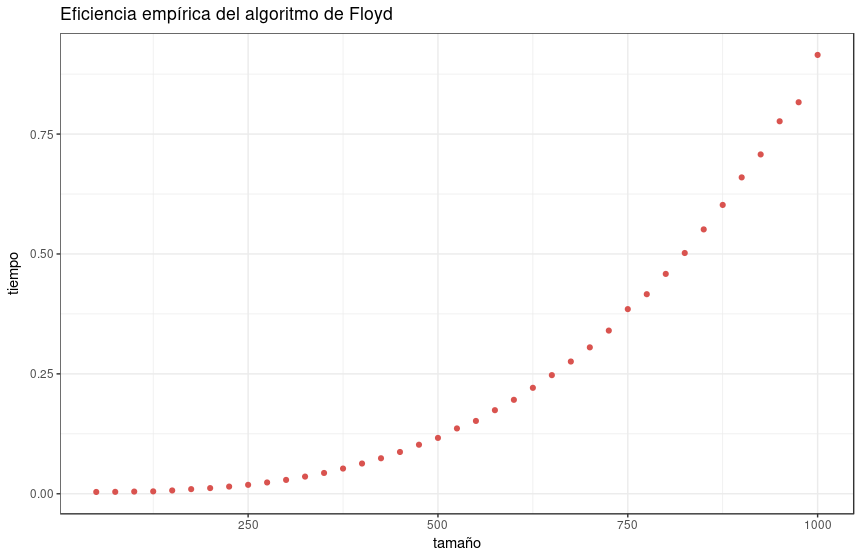
\includegraphics[width=\textwidth]{Floyd_empirica.png}
	\caption{Eficiencia empírica del algoritmo de Floyd.\label{floydemp}}
\end{figure}

Para tomar estos tiempos tuvimos que reducir un poco los tamaños en comparación con los algoritmos de búsqueda.

\pagebreak
\subsection{Algoritmo de orden $2^n$.}

\begin{figure}[!hbp]
	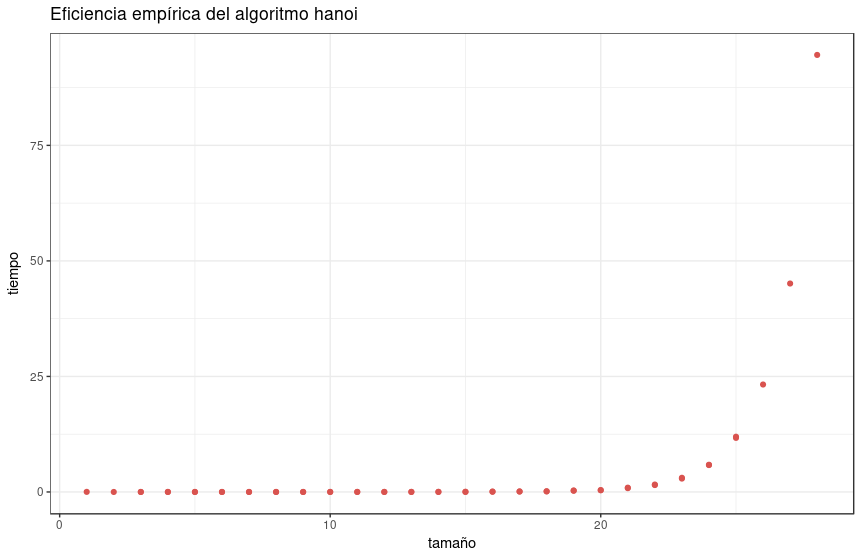
\includegraphics[width=\textwidth]{hanoi_empirica.png}
	\caption{Eficiencia empírica del algoritmo de Hanoi.\label{hanoiemp}}
\end{figure}

EL principal problema que encontramos con este algoritmo fue que, por su orden de eficiencia, era imposible ejecutarlo para tamaños superiores a 50 elementos en tiempos razonables, por eso tomamos tiempos hasta 25 elementos. Para llegar a esta conclusión fuimos intentando ejecutar tamaños de 100, 90, 80... elementos hasta que vimos que con 20 se ejecutaba (tras unos minutos). 
\pagebreak
\section{Eficiencia híbrida.}
Hemos realizados los distintos ajustes de los tiempos anteriormente comentados con gnuplot tal y como se indica en el guión y hemos guardado algunas capturas de pantalla de los resultados obtenidos. Las gráficas obtenidas son las siguientes:

\subsection{Algoritmos de orden $nlogn$.}


\begin{figure}[!hbp]
	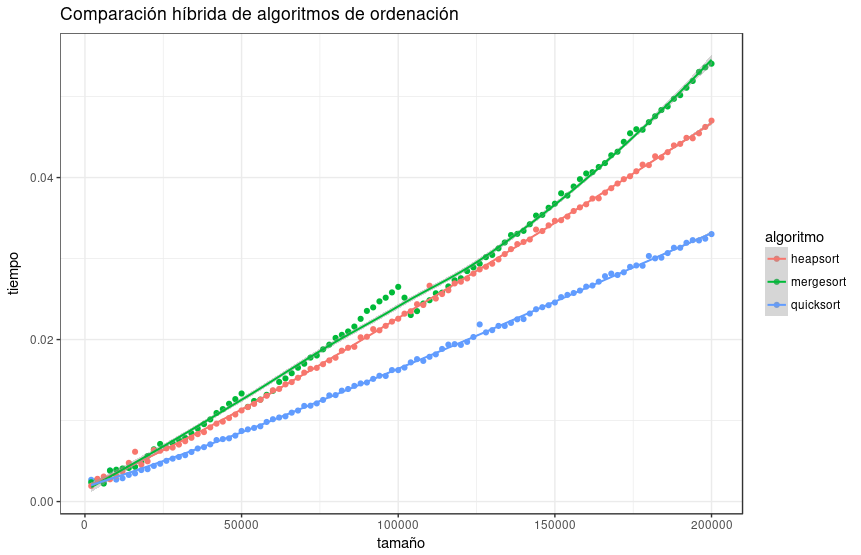
\includegraphics[width=\textwidth]{hibridaor.png}
	\caption{Eficiencia híbrida de los algoritmos de ordenación de orden $nlogn$.\label{hibridaor1}}
\end{figure}

    Aquí podemos ver como aunque los algoritmos tengan el mismo análisis O, no se ajustan a la misma gráfica, sino que hay algoritmos más eficientes que otros. 
    Hemos ajustado los tiempos a la función $f(n) = a*nlog(b*n)+c$. Los datos del ajuste de los 3 algoritmos son los siguientes:

	\VerbatimInput{ajustes}
	
	Luego las funciones que se ajustan a los tiempos de los distintos algoritmos son:
	\begin{itemize}
		\item Heapsort: $f(n) = 4.34068*10^5*nlog(0.901865*n)+0.00511096$
		\item Quicksort: $f(n) = 3.02225*10^9*nlog(0.901855*n)+0.00171908$
		\item Mergesort: $f(n) = 3.02225*10^{9}*nlog(0.901855*n)+0.00171908$
	\end{itemize}

\pagebreak
\subsection{Algoritmos de orden $n^2$.}


\begin{figure}[!hbp]
	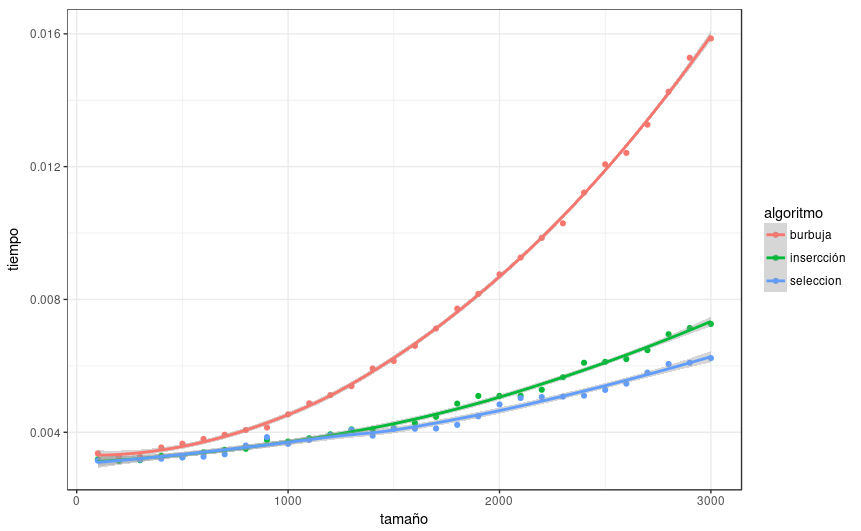
\includegraphics[width=\textwidth]{hibridaor2.png}
	\caption{Eficiencia híbrida de los algoritmos de ordenación de orden $n^2$.\label{hibridaor2}}
\end{figure}

\begin{figure}[!hbp]
	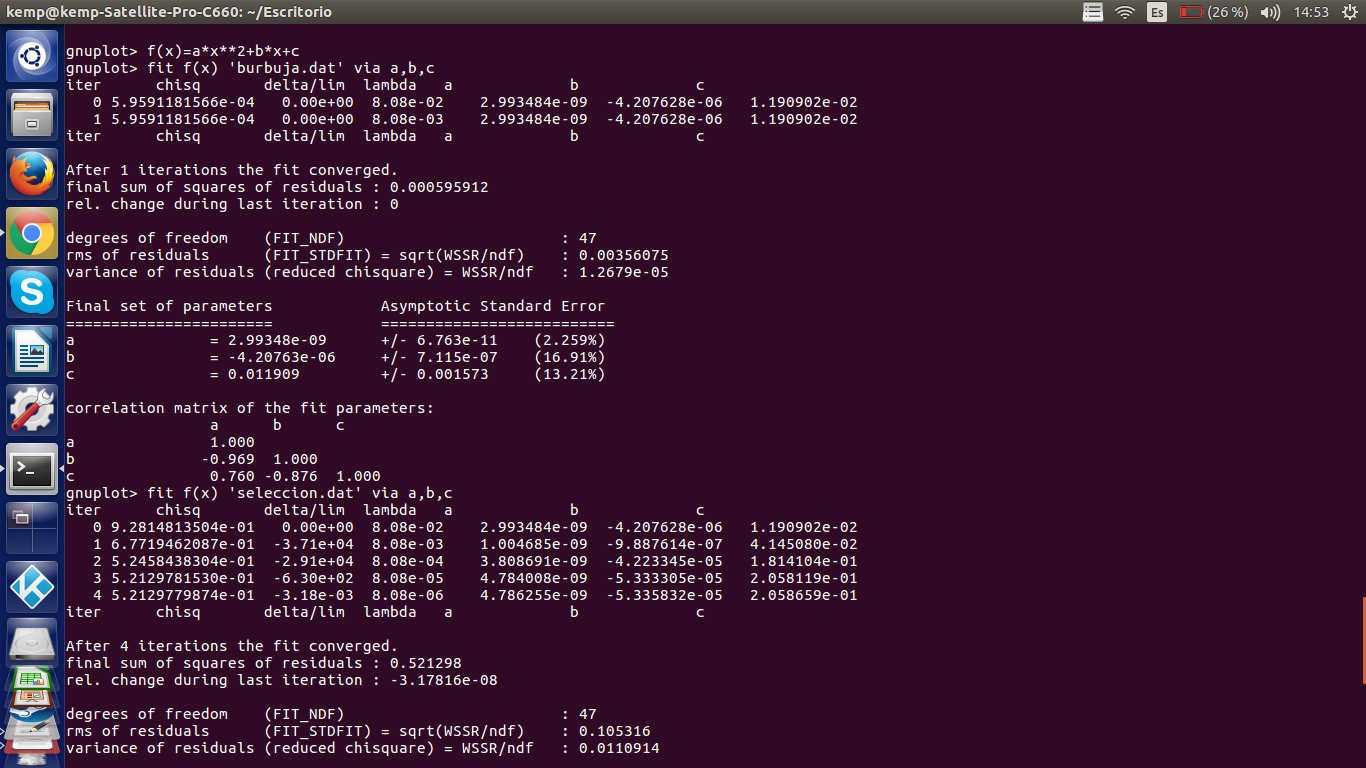
\includegraphics[width=\textwidth]{gnuplot_burbuja.png}
	\caption{Ajuste burbuja\label{ajust1}}
\end{figure}
\begin{figure}[!hbp]
	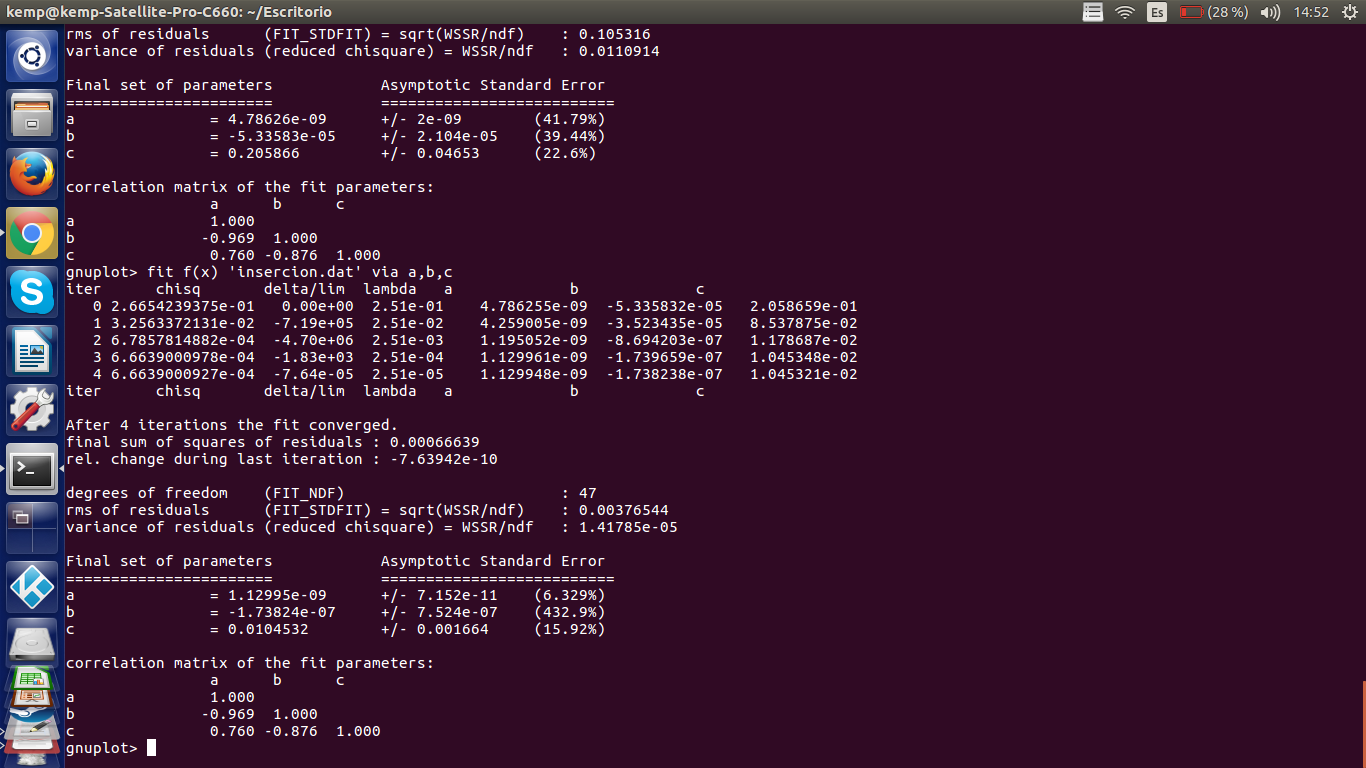
\includegraphics[width=\textwidth]{gnuplot_insercion.png}
	\caption{Ajuste inserción\label{ajust2}}
\end{figure}
\begin{figure}[!hbp]
	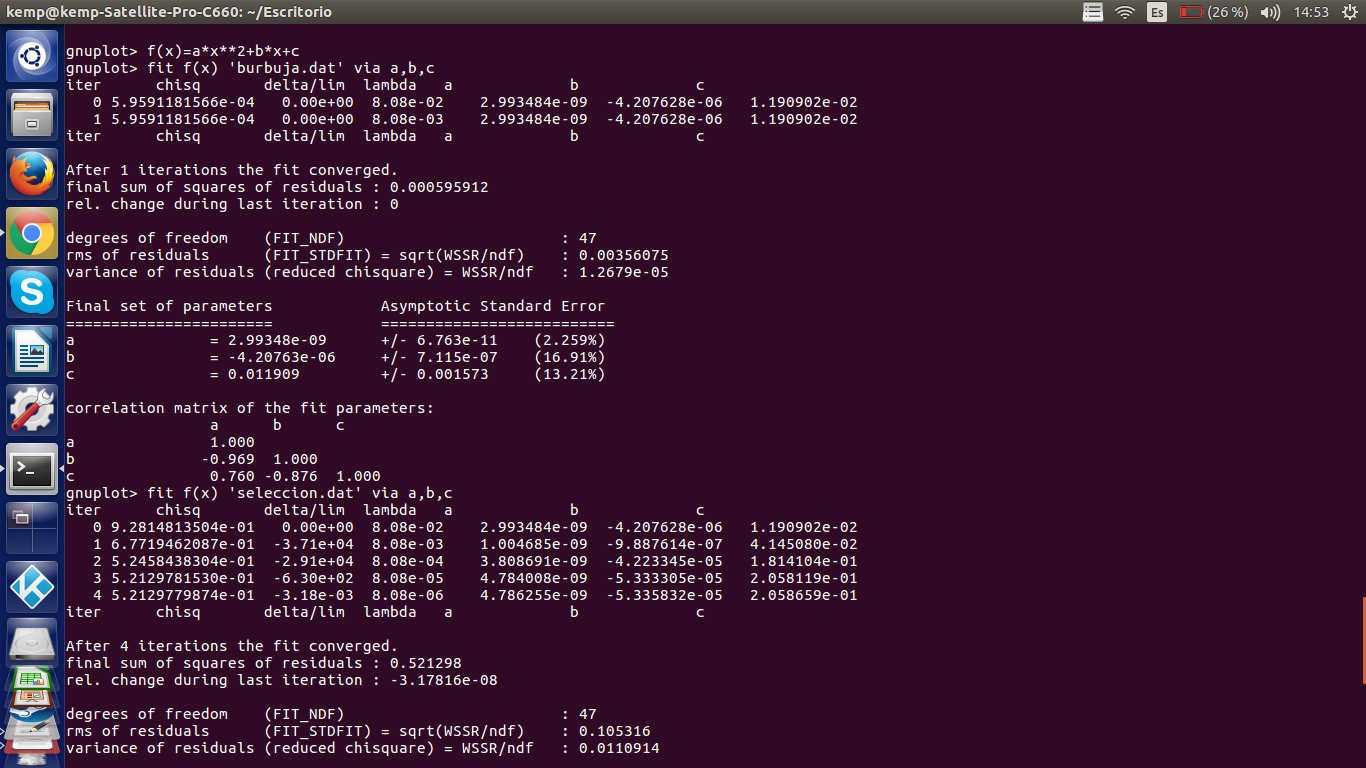
\includegraphics[width=\textwidth]{gnuplot_burbuja.png}
	\caption{Ajuste selección\label{ajust3}}
\end{figure}

\pagebreak
\subsection{Algoritmo de orden $n^3$.}

Aquí podemos ver perfectamente una parábola, que cuantos más datos más se parecerá a una parábola $n^3$. Los datos del ajuste están en la misma imagen:
\begin{figure}[!hbp]
	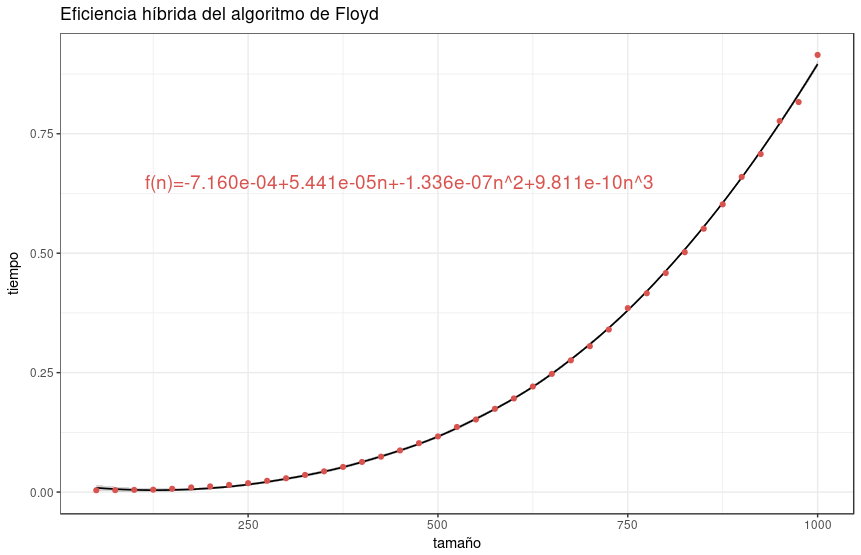
\includegraphics[width=\textwidth]{floyd_hibrido_formula.png}
	\caption{Eficiencia híbrida del algoritmo de Floyd.\label{ffloyd}}
\end{figure}
\pagebreak
\subsection{Algoritmo de orden $2^n$.}
	 Podemos ver como sigue la filosofía de un algoritmo exponencial, a partir de un número de datos, en este caso 28, el algoritmo se hace prácticamente inútil, ya que el tiempo que tarda es demasiado. Los datos de la regresión son los siguientes:

\begin{figure}[!hbp]
	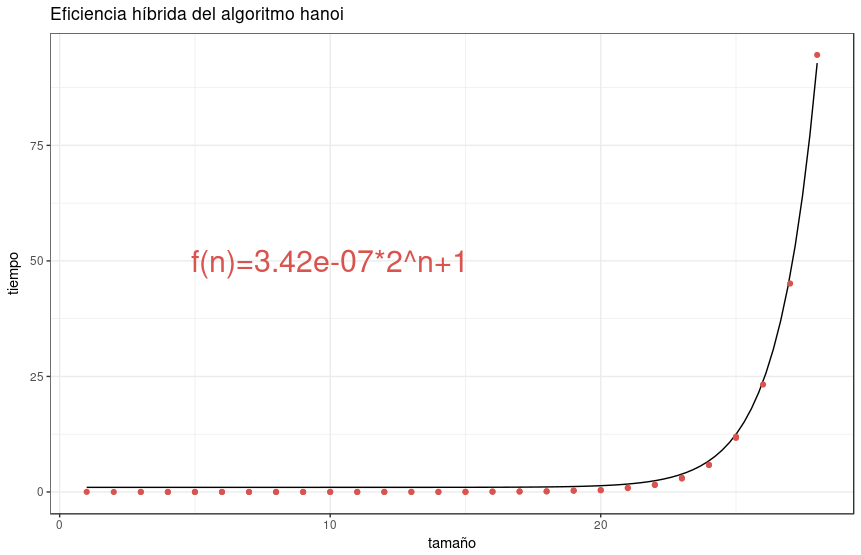
\includegraphics[width=\textwidth]{hanoi_hibrido_formula.png}
	\caption{Eficiencia híbrida del algoritmo de las torres de Hanoi{hhanoi}}
\end{figure}
\begin{figure}[!hbp]
	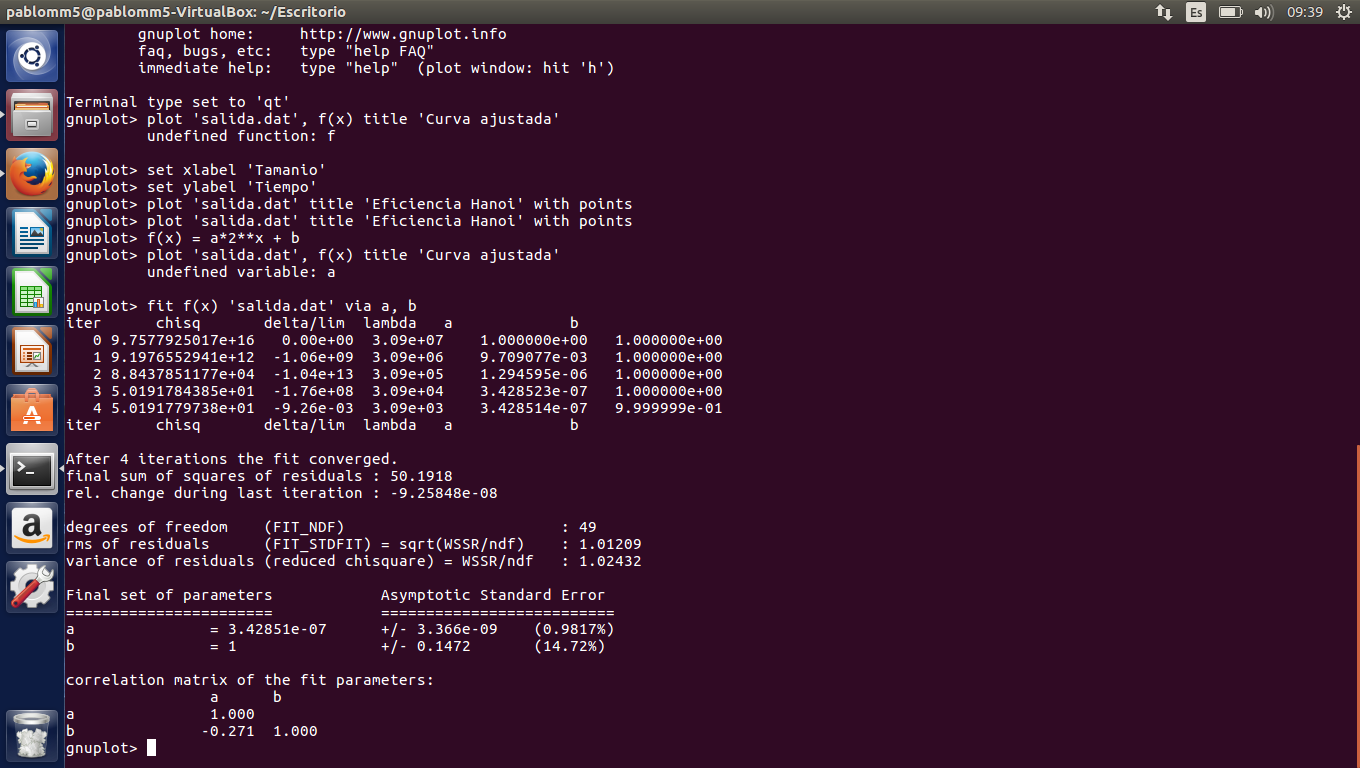
\includegraphics[width=\textwidth]{gnuplot_hanoi.png}
	\caption{Ajuste Hanoi\label{ajust4}}
\end{figure}

\pagebreak
\section{Otros análisis}
\subsection{Burbuja con distintas optimizaciones.}
En la siguiente gráfica se ve claramente como con diferentes optimizaciones del compilador la eficiencia cambia. Sin optimización, lógicamente, el algoritmo es menos eficiente. Con optimización 1, el algoritmo ya va tardando menos, sobre todo cuando el número de datos aumenta. Y finalmente, con optimización 2, la eficiencia mejora considerablemente, de manera que se empieza a notar aunque el número de datos no sea tan significativo.
\begin{figure}[!hbp]
	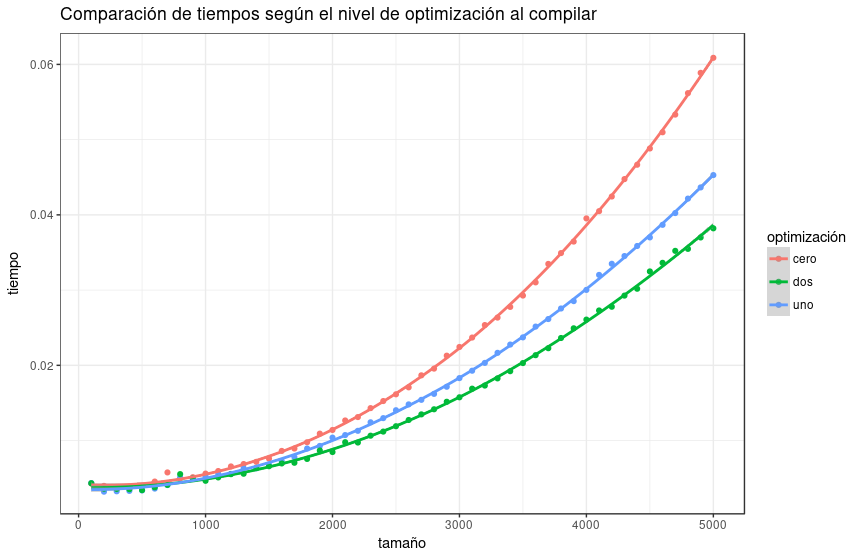
\includegraphics[width=\textwidth]{burbujaopt.png}
	\caption{Comparación de ejecuciones del algoritmo burbuja según la optimización.\label{opt}}
\end{figure}
\pagebreak
\subsection{Comparación del Heapsort en distintos ordenadores.}
\begin{figure}[!hbp]
	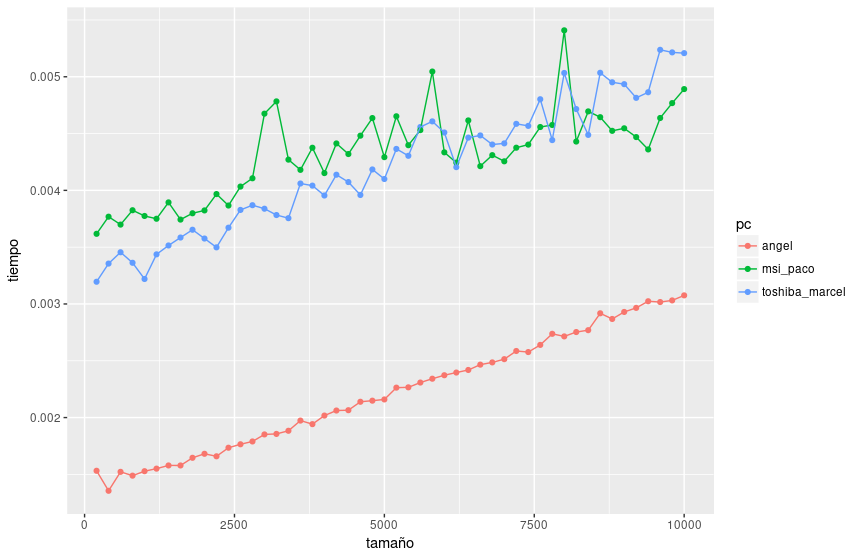
\includegraphics[width=\textwidth]{ordenadores.png}
	\caption{Comparación de ejecuciones del algoritmo  heapsort con distintos ordenadores\label{ordenadores}}
\end{figure}
Hemos probado a ejecutar el algoritmo heapsort en tres ordenadores distintos. Mientras que en el msi y el toshiba los tiempos eran muy similares, el tercer ordenador, un Lenovo i7, ha obtenido tiempos mucho más rápidos (ordenador etiquetado como ángel)
\pagebreak
\subsection{Mal ajuste de la función de Hanoi}
Hemos comprobado qué ocurriría si hacemos un ajuste a los tiempos de un algoritmo con una función que no se corresponde a su eficiencia teórica, concretamente hemos ajustado el algoritmo de las torres de Hanoi con $f(x)=x+x^2$. El resultado:
\begin{figure}[!hbp]
	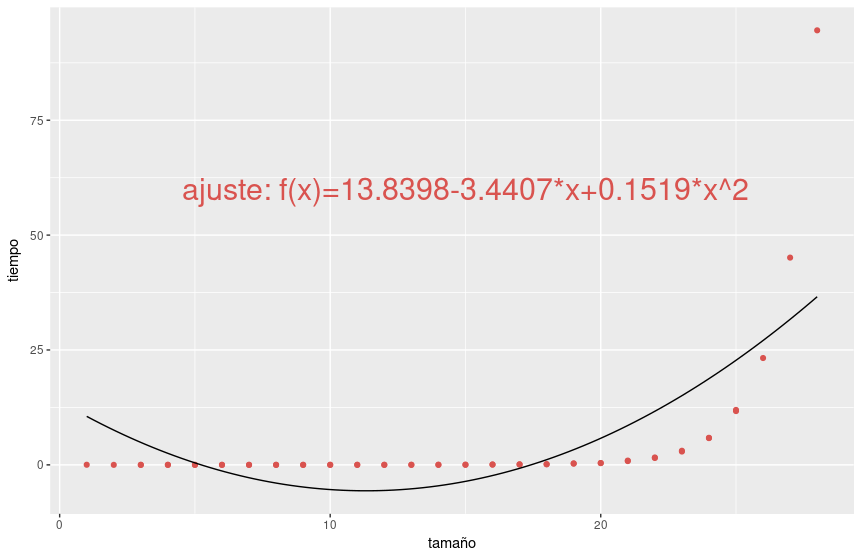
\includegraphics[width=\textwidth]{hanoibad.png}
	\caption{Mal ajuste de Hanoi \label{hanoibad}}
\end{figure}

\subsection{Comparación de Heapsort y Quicksort en el peor de los casos del Quicksort}
Nos ha parecido interesante hacer una comparación especial de los algoritmos de ordenación quicksort y heapsort ya que, aunque el primero da mejores tiempos por lo general, hay casos (cuando el vector a ordenar está parcialmente ordenado) en los que los tiempos empeoran hasta el punto de llegar a obtener tiempos de orden $n^2$. No así el heapsort que, aunque da resultados generalmente peores que el quicksort, se mantiene en $nlogn$ sea cual sea el estado del vector.

\begin{figure}[!hbp]
	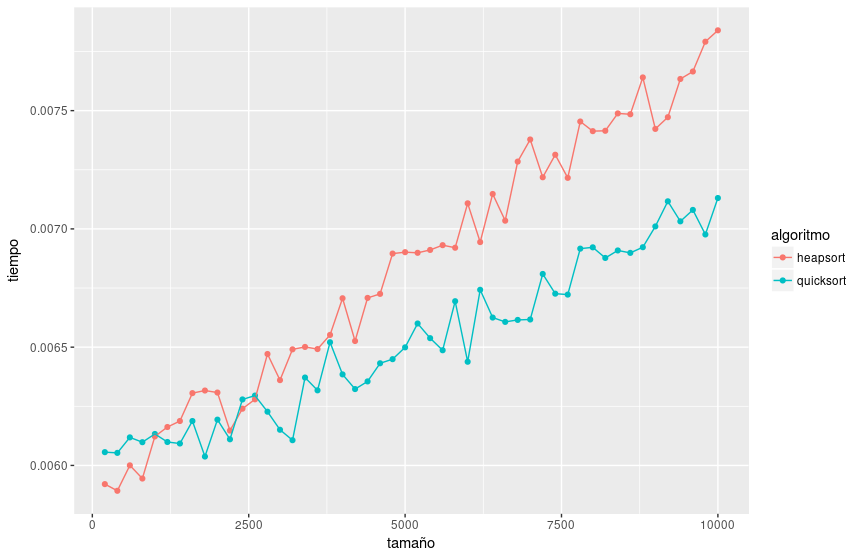
\includegraphics[width=\textwidth]{NOordenadosquickheap.png}
	\caption{Comparación del quicksort y el heapsort con vectores aleatoriamente ordenados\label{ref1}}
\end{figure}

\begin{figure}[!hbp]
	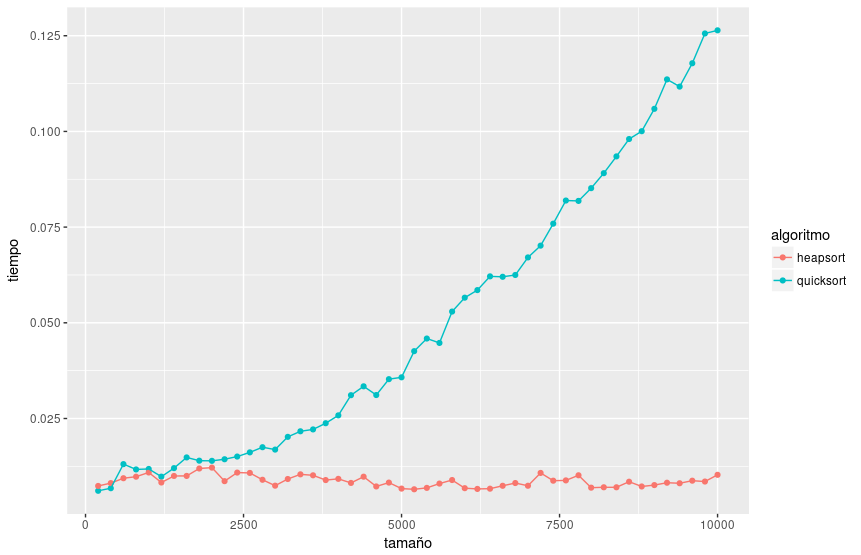
\includegraphics[width=\textwidth]{heapsort_quicksort_ordenados.png}
	\caption{Comparación de quicksort y el heapsort con el vector parcialmente ordenado (u ordenado) \label{ref2}}
\end{figure}

\pagebreak
\section{Ordenador usado para medir los tiempos}

\begin{figure}[!hbp]
	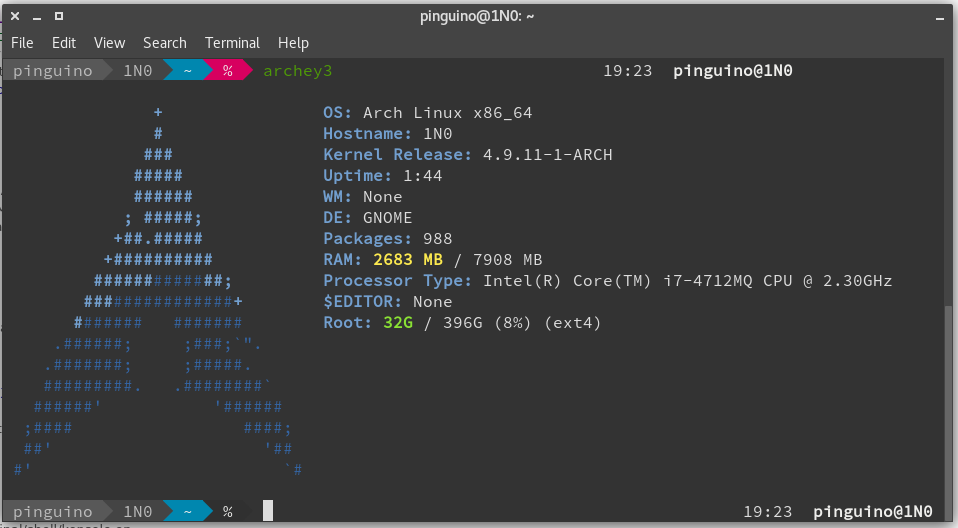
\includegraphics[width=\textwidth]{arch.png}
	\caption{ARCH LINUX\label{arch}}
\end{figure}




\end{document}